\section{Experiment planning}

\begin{frame}{fishVR V2 Concept}{}
	\centering
	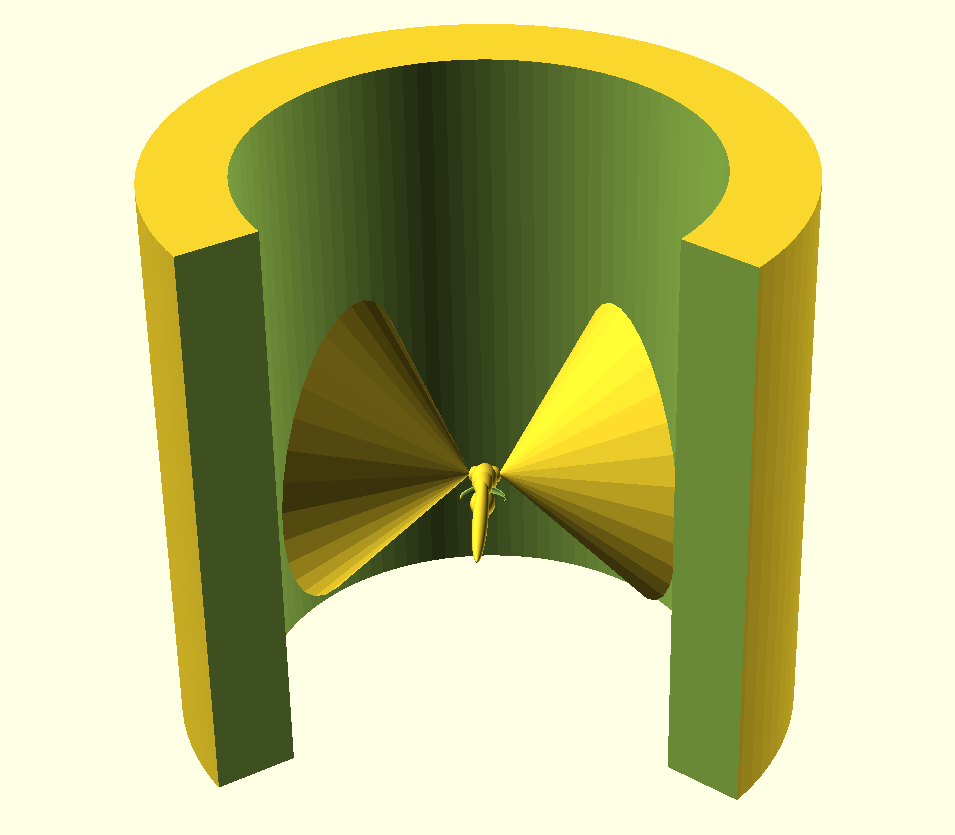
\includegraphics[height=0.9\textheight]{media/zfish_render}\nakedfootnote{https://github.com/BadenLab/Zebrafish-visual-space-model}
\end{frame}{}

\begin{frame}{fishVR V2 Reality}{flexible OLED display}
	\centering
	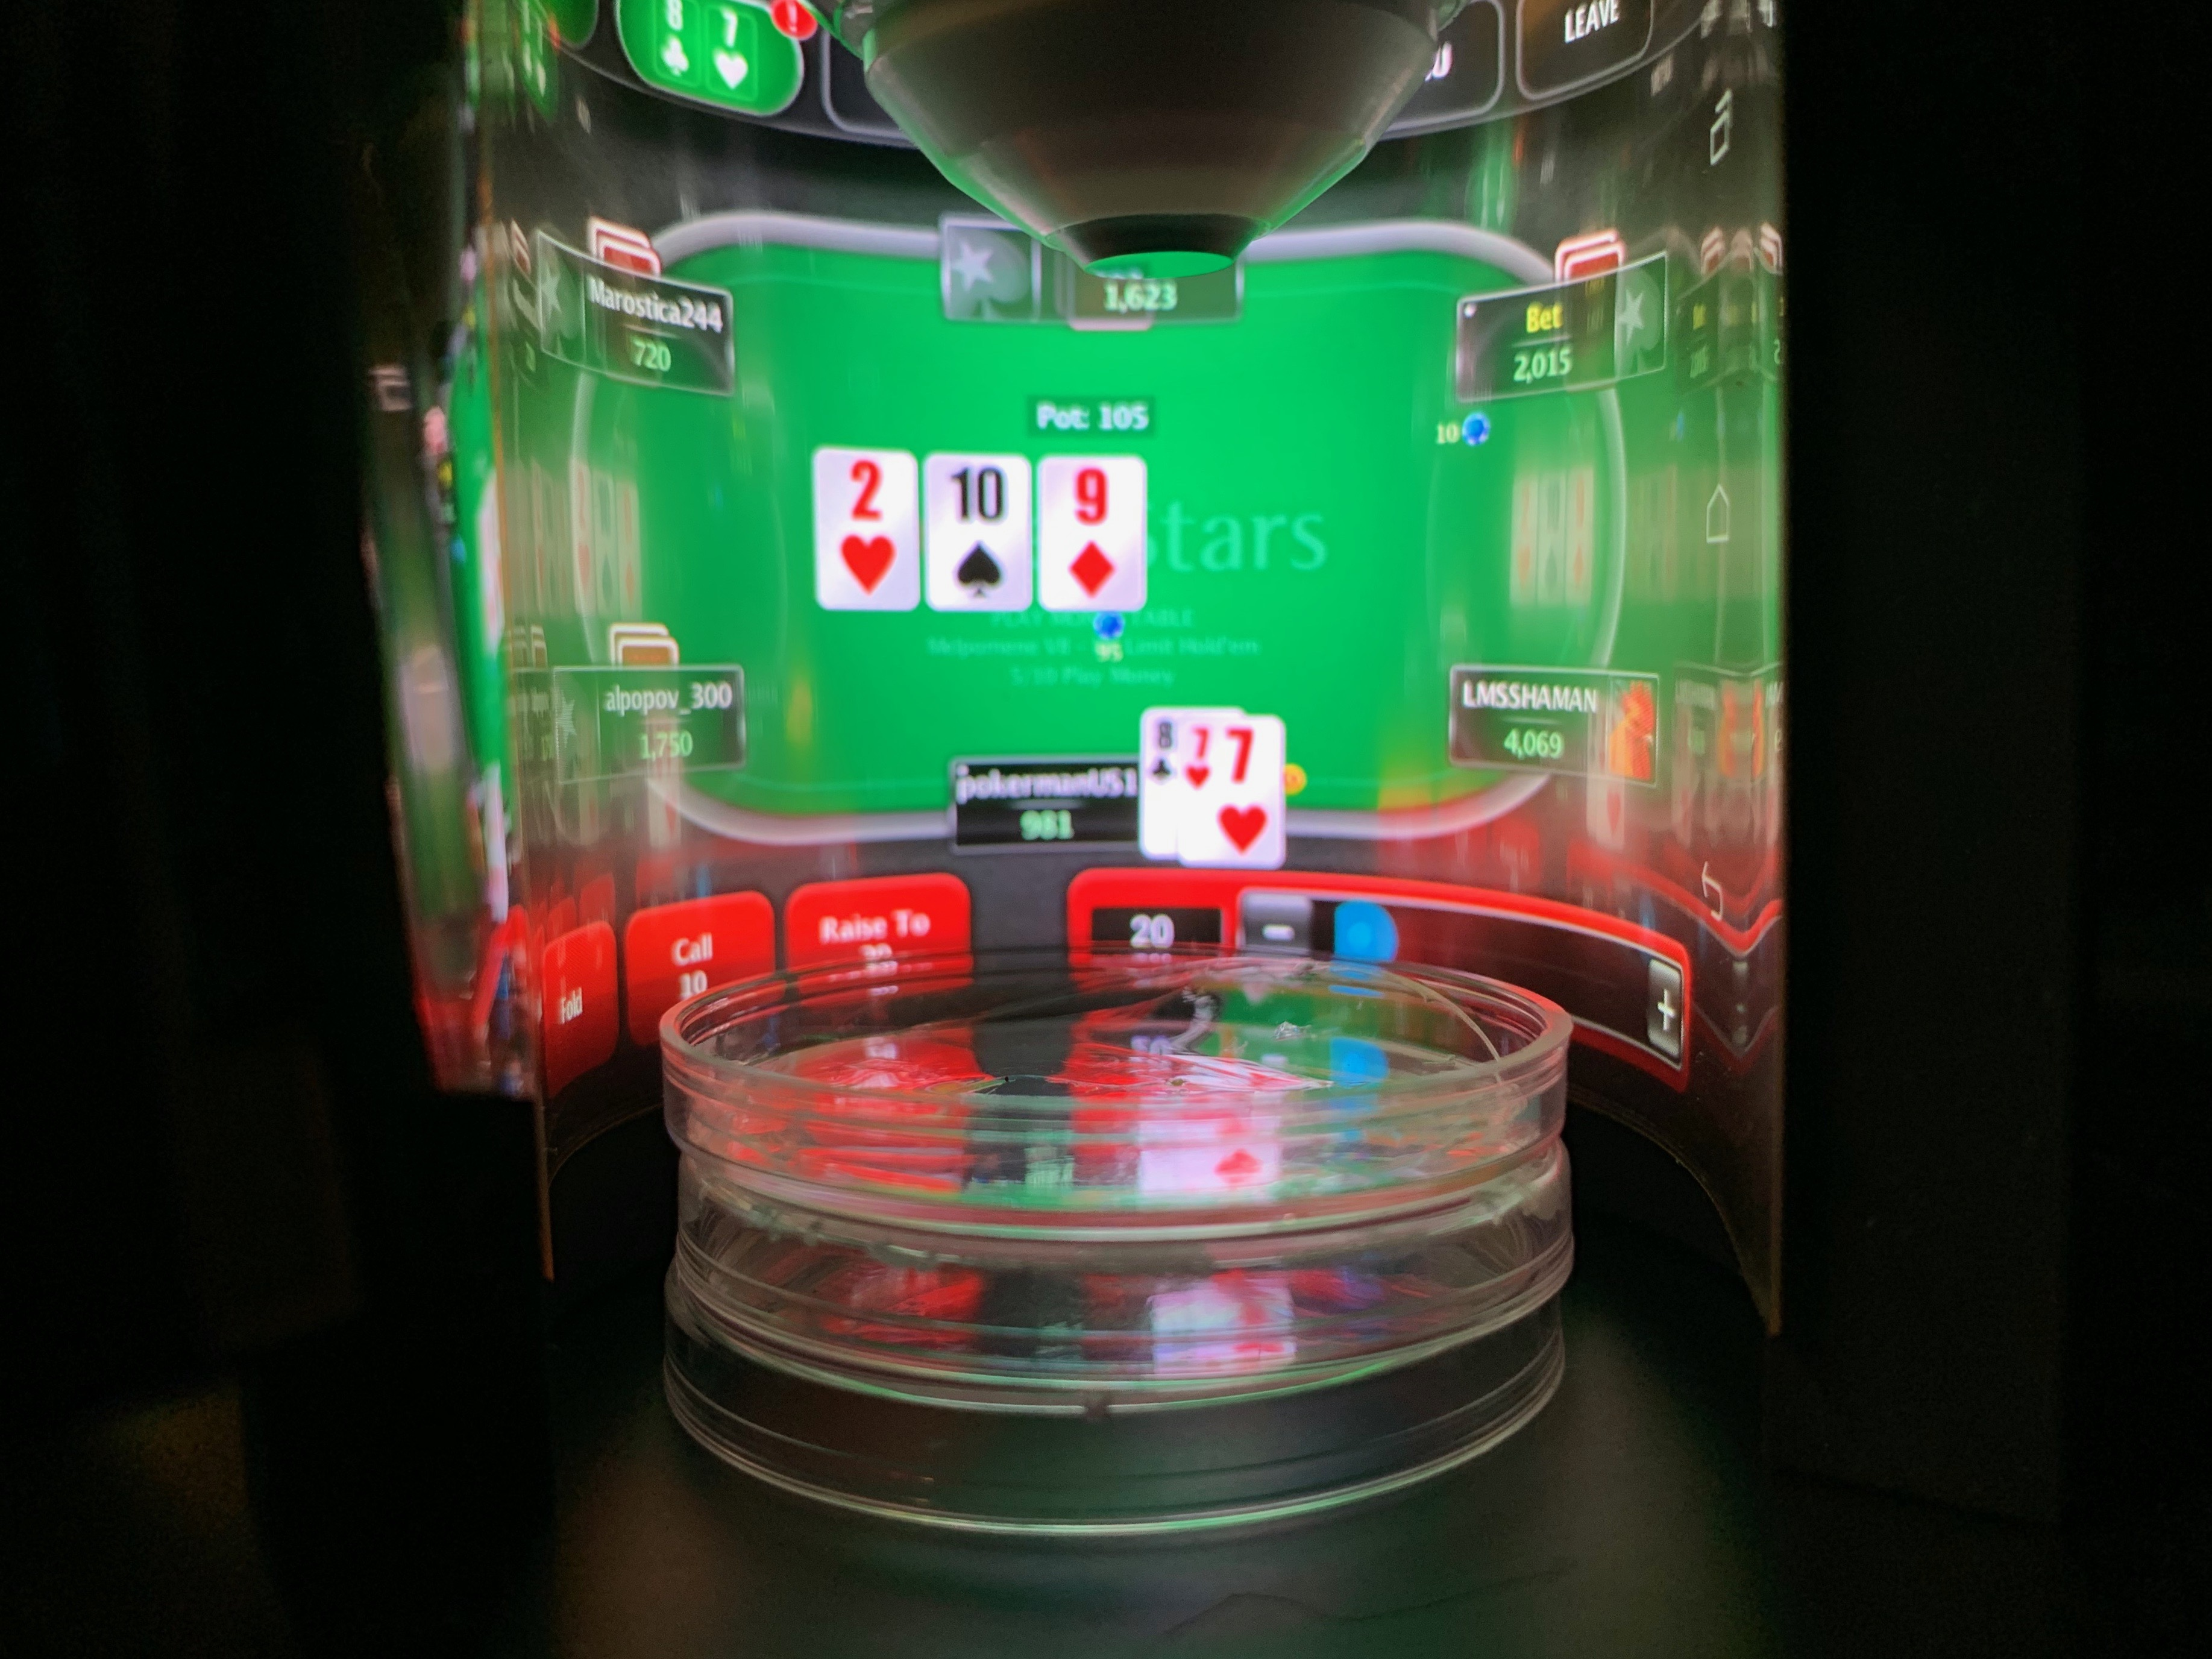
\includegraphics[height=0.9\textheight]{media/poker-fish}
	\note{Unlike LCD and projector, can completely turn off green light}
\end{frame}{}

\begin{frame}{Next steps (feedback welcome!)}{}
	\centering
	\begin{itemize}
		\item Focus on calcium imaging for immediate future \& analyze behavior from optomotor response data
		\item Contextualized passive coping: Aaron's regime with colored queue to indicate if shock is escapable
		\item Pursue initial optogenetic experiments with predicting dynamics recovery after region-wide NpHR inhibition
		\item Outcross F0s in ~1-2 weeks to see if stable F1 emerges
	\end{itemize}
\end{frame}{}

\begin{frame}{Acknowledgements}{}
	\centering
	\begin{columns}[t]
    \column{0.5\textwidth}
			\begin{itemize}
				\item Aaron
				\item Matt LB
				\item Noah
				\item Susanna
				\item Ritchie
				\item YoungJu
				\item Toni
				\item John
				\item Ailey
				\item Sean
				\item Misha, Brian, Ted
			\end{itemize}
    \column{0.5\textwidth}
			\begin{itemize}
				\item Karl
				\item Shaul
				\item Charu
				\item Sally
				\item Cynthia
			\end{itemize}
  \end{columns}
\end{frame}{}
